\documentclass[12pt]{article}   %  [titlepage]   \and
\usepackage{amsmath}
\usepackage[utf8]{inputenc}
\usepackage[T1]{fontenc}
\usepackage[danish]{babel}
\renewcommand{\rmdefault}{ptm}
\usepackage[pdftex]{graphicx}
\usepackage{multirow}

\title{IT-løsning til Tolkeservice}
\author{Omar Khalidan - [xx-xx-xx]\\
     Morten Trolle Nielsen - [14-06-79]\\ \\
    Instruktor: Andreas Frisch\\ \\
Projekt i systemudvikling 2014 (ProjDat2014)}

\begin{document}
\maketitle
\thispagestyle{empty}
\newpage
\tableofcontents
\newpage

\section{Abstract}
Dette er anden delrapport i faget Systemudviking. Vores udgangspunkt er første
delrapport, som vi her udvikler og udbygger. Vi vil foresætte arbejdet med og
præsentationen af den IT-løsning, som vi har udviklet til kunden; tolkeservicen
K. Translation. Specielt vil vi fokusere på modelleringen af systemet. Vi vil 
præsentere anvendelsesområdet og problemområdet; både med tekst og UML-diagrammer.
Det skal resultere i en bedre og umiddelbar forståelse af vores påtænkte it-løsning.
Derefter vil vi også med afsæt i første delrapports kravspecificering videreudvikle
denne og se på de funktionelle og nonfunktionelle krav. Vi vil tage modelleringen
et skridt videre ved hjælp af use-cases, så vi kan understøtte vores modellering med
konkrete eksempler på brug af systemet. \\
Vi vil afslutte denne anden delrapport med to korte referater og efterfølgende
analyse og perspektivering af de to artikeler, der er et krav til rapporten.\\
Vi er selv førsteårs datalogistuderende ved Københavns Universitet, og det
forudsættes, at læseren befinder sig på samme læringsniveau eller højere, idet
der undervejs vil forekomme adskillige fagspecifikke termer. 

\newpage

\section{Problemformulering}

\emph{”Hvordan konstruerer man et bookingsystem til en tolkevirksomhed, som
formindsker tidsspilde og fejl ? Og hvordan kan dette gøres på en brugervenlig
måde, så virksomhedens samarbejdspartnere enkelt og simplet kan tilgå systemet 
uden tidsspilde ?”}\\

Tolkeservicen K. Translation er et lille, enmands tolkebureau med speciale i arabiske 
sprog. Indehaveren af bureauet er , og hun er som sagt både leder og eneste
medarbejder i foretagendet. Hendes kunder er offentlige myndigheder som
politiet og anklagemyndigheden og private aktører som advokatbureauer og
forskellige virksomheder. Disse instanser kontakter K. Translation, når de har
behov for en tolk til konkrete sager eller ved andet forefaldende
tolkearbejde, og der laves en aftale. Det kan både være aftaler to eller tre uger 
ude i fremtiden, eller det kan være aftaler med kortere frist ved mere presserende 
sager.\\
K. Translation (KT) har i længere tid ønsket et it-system, som kan
afhjælpe lidt af den daglige travle arbejdsbyrde. Derfor tog ejeren af KT
kontakt til os, og anmodede om et møde omkring dette problem. Det første møde fandt 
sted fredag den 21. marts, og vi blev enige om at begynde et samarbejde, der
skal resultere i et færdigt kalender- og bookingssytem til KT og KT's kunder.
Kunden præsenterede os for en liste af de funktioner, som hun ønsker, at det nye system
skal kunne levere. For det første ønskes der en hjemmeside, hvor KT's kunder
kan logge på systemet med deres EAN-nummer. Da vi bl.a. snakker om offentlige
myndigheder som politi og anklagemyndighed, skal login systemet fremstå
professionelt og sikkert. Der skal være en tilhørende database indeholdende
alle KT's kunder, og det skal være muligt løbende at tilføje kunder til
databasen. \\
Når KT's kunde har logget på systemet, skal vedkommende præsenteres for en
kalender opslået på dags dato med mulighed for visning af de næste to til tre
uger. Det er KT's holdning og erfaring, at der ikke forekommer aftaler længere
end tre uger ude i fremtiden; derfor denne begrænsning. KT's kunde skal i
kalenderen kunne se alle de tidspunkter, hvorpå det er muligt at booke en
aftale med K. Translation. Disse ledige tidspunkter kan evt. markeres med
grønt. Allerede indgåede aftaler markeres med rødt for at tydeliggøre
denne forskel. Når KT's kunde har besluttet sig for en dato og et tidspunkt,
taster vedkommende dette ind i systemet, og aftalen gemmes i databasen og
vises herefter i kalenderen. Det er vigtig for KT's ejer, at hendes
samarbejdspartnere ikke skal bruge alt for lang tid på at booke en aftale, så
enkelhed og intuitivitet skal prioriteres højt.\\

\section{Projektaftale}
Inden vi fortsætter med modelleringen og designet af systemet, vil vi beskrive
præcist, hvilke krav og forventninger kunden K. Translation har til vores
endelige løsning. Vi har delt den følgende kravspecifikation op i to dele:
high-level funktionelle krav, som dækker samspillet mellem anvendelsesområdet og
kalender- og bookingsystemet uden implementeringsspecifikke detaljer. Og
nonfunktionelle krav, der dækker over ikke direkte funktionelle aspekter som
bl.a. brugervenlighed og pålidelighed. Idet kravspecifikationen senere danner
grundlag for afprøvningen af systemet, er det vigtigt, at den er ``komplet,
konsistent, entydig og korrekt.''\cite{oose}[p.~122] \\

\subsection{Funktionelle krav}
På det første kundemøde beskrev indehaveren af K. Translation, hvilke
forventninger og ønsker hun havde til det færdige produkt: et integreret
kalender og bookingsystem. Det dannede grundlaget for kravspecifikationen, som
nu udgører rammerne indenfor hvilke, vi udvikler systemet. De funktionelle
krav kan ses i den efterfølgende liste.\\


\rule{120mm}{1mm}
\begin{itemize}
\item K. Translation ønsker en it-løsning, der indeholder en kalender og et
	bookingsystem, som af bureauets kunder kan tilgås over intetnettet.
\item På hjemmesiden skal KT's kunder præsenteres for en login menu, hvor de
	logger på systemet med virksomhedens eller institutionens EAN-nummer
	og et selvvalgt password. 
\item Efter succesfuldt login tilgår kunden kalenderen. Det skal være muligt
	for kunden at søge i kalenderen efter ledige tidspunkter udfra kriterier 
	som dato og klokkeslet. 
\item Der skal sendes en bekræftende email tilbage til kunden, efter at
	vedkommende har booket en tid i kalenderen. Det blev af KT foreslået,
	at kunden modtager et vCard   
\item Det skal være muligt for K. Translation løbende at tilføje flere kunder 
	eller samarbejdspartnere til databasen. 
\item KT's indehaver vil gerne kunne overføre sine private aftaler fra en
	ekstern kalender til vores kalendersystem. Hun forestiller sig en form
	for synkronisering, men vi har fra start gjort hende det klart, at
	dette måske ligger udover det mulige. Se evt. afsnittet om
	projektplan, hvor vi diskuterer prioriteringer. 
\end{itemize}
\rule{120mm}{1mm}
\vspace{0.5cm}

Vi har i samarbejde med KT udviklet den ovenstående liste af funktionelle
krav, men KT havde fra start et godt billede af, hvilke funktioner og egenskaber det
færdige produkt skulle indeholde. Sammen identificerede vi først de aktører, der skal 
kunne tilgå systemet; altså i virkeligheden anvendelsesområdet. Derefter
beskrev KT's indehaver en række typiske scenarier fra hendes daglige arbejde,
hvor kunder til bureauet booker en tid hos tolkeservicen. Udfra disse
scenarier kunne vi opstille flere af de funktionelle krav, og dette arbejde
kulminerer iøvrigt senere i rapporten i afsnittet omhandlende use-cases. Vi
synes, at de funktionelle krav på en god og dækkende måde beskriver de
ønsker, som K. Translation har til det færdige program. Det skulle være
muligt at teste, om vores løsning lever op til alle ovenstående krav, når
systemet senere skal valideres på baggrund af kravspecifikationen.  \\ 



\subsection{Non-funktionelle krav}
Indehaveren af K. Translation kom også med nogle forventninger og ønsker, som
ikke umiddelbart hører til systemets funktionelle egenskaber. Det er bl.a.
forventninger om brugervenlighed, pålidelighed og andre svært verificerbare
egenskaber. Disse ønsker har vi samlet her i afsnittet med nonfunktionelle
krav sammen med mere implementeringsspecifikke detaljer. Den efterfølgende liste
indeholder de nonfunktionelle krav til systemet.\\

\rule{120mm}{1mm}
\begin{itemize}
\item Kalender og bookingsystemet skal placeres på en hjemmeside.
\item Hjemmesiden skal indeholde K. Translations kontaktinformationer. Der er
	ikke stillet særlige krav til designet udover, at det skal være enkelt
	og intuitivt, så personer uden store it-forudsætninger kan navigere på
	siden og booke en tid.
\item Alle brugere skal kunne tilgå systemet med en almindelig web browser som
	Internet Explorer, Firefox eller Google Chrome.
\item KT's kunder skal hurtigt og uden mulighed for misforståelse kunne skelne ledige
	tidspunkter i kalenderen fra optagede. Derfor skal ledige tidspunkter
	markeres med grøn skrift eller farve, og allerede indgåede aftaler
	markeres med rødt.\footnote{Der kan godt argumenteres for, at dette
		punkt er en funktionel egenskab ved systemet, men vi har
		placeret det under de nonfunktionelle krav, da bl.a. omhandler
	brugervenlighed og implementeringen.}
\item K. Translation ønsker den letteste og billigste implementering og
	hosting af systemet. Hun vil have et system, der ikke kræver løbende
	vedligeholdelse, men som bare ``kører og passer sig selv''.   
\item Da KT's kundegrundlag bl.a. udgøres af offentlige myndigheder og
	ministerier, må der ikke være tvivl om systemet integritet og
	pålidelighed.
\item Der ønskes præcis og let forståelig dokumentation af systemet. 
	Især ønsker indehaveren dækkende, enkle manualer i tilfælde af, at hun
	selv må stå for den løbende vedligeholdelse af systemet og i tilfælde
	af svigt og andre fejl.
\item Kalendersystemet og backend databasen må ikke tabe data eller aftaler.
\end{itemize}
\rule{120mm}{1mm}
\vspace{0.5cm}

Som det fremgår, vil flere af de nonfunktionelle krav være svært verificerbare. 
Det er meget svært at fastslå med nogen som helst sikkerhed, hvornår en bruger
opfatter en hjemmeside som enkel, intuitiv og let at overskue. Man kan stille
parametre op, fastsætte gennemgående regler for designet og bruge afprøvede
metoder, men der kan alligevel ikke gives nogen garantier. Derfor vil vi også
i en senere rapport bruge tænke-højt-forsøg for at få en ide om, hvor godt
eller dårligt vores design er i forhold til disse egenskaber. Andre af de
nonfunktionelle krav udspringer af manglen på it-kompetancer i bureauet og af
fraværet af en systemadministrator. Dette betyder højest sandsynligt, at vi 
placerer det færdige system hos en udbyder af serverplads, da KT i så fald kommer 
til at stå for et minimum af systemvedligehold. Det vil også være den billigste
løsning, da anskaffelsen af en server, strøm og evt. køling til en sådan vil
resultere i en betragtelig udgift. \\
Da belastningen af systemet ikke forventes at blive særlig høj, kar KT. ingen 
performancemæssige krav til vores løsning. Der er ingen tids kritiske
brugerfunktioner, og risikoen for samtidig brug af kalenderen må forventes at
være minimal. Man kunne godt forestille sig to kunder, der vil booke den samme 
tid i kalenderen med race condition og deadlock til følge, men backend
databasens transactionindstillinger burde kunne håndtere dette
tilfredsstillende. Pålidelighed er på den anden side et vigtigt og naturligt
issue, da K. Translation ikke kan acceptere, at aftaler tabes eller
forsvinder. \\ 

\section{Projektplan}
Adskillige forelæsninger i Systemudviklingskurset har handlet om agil
projektledelse og systemudvikling. Vi har fundet en sådan iterativ og
inkremental tilgang til projektet spændende, og kunne derfor godt tænke os, at
systemudvikle inden for rammerne af de agile principper, som vi bl.a. har
stiftet bekendsskab med i artiklen ``Jeff Sutherland's Scrum
Handbook''\cite{scrum}. Det vil dog ikke være muligt, at gennemføre projektet
i komplet overensstemmelse med Scrum og alle de agile regler. For det første
vil det betyde, at vores kunde skal afse betydelig mere tid til projektet,
end hun umiddelbart har planlagt, hvis hun løbende skal opdate ``Product
Backlog'' og deltage i prioriteringsmøder ved hver sprints begyndelse.
Derudover vil det ikke være realistisk, at vi selv holder daglige Scrum møder,
og at vi kan levere al den dokumentation et virkeligt Scrum forløb
forudsætter som f.eks. de daglige overslag over vores egne fremskridt i forhold
til de påtagede opgaver i den aktuelle sprint. Derfor vil vi slække på nogle af 
reglerne, og vi håber at kunne gøre det uden at bevæge os alt for langt væk fra 
den virkelige agile Scrum systemudvikling.\\
I stedet for de daglige estimeringer over projektets fremadskriden, har vi
valgt at nøjes med et overordnet burndown diagram for hele projektet. Se figur
\ref{fig:bd}. (Et brundown diagram for en enkelt sprint vil være magen til,
men værdierne på førsteaksen vil være dage i stedet for uger, og værdierne på
andenaksen vil være mindre). 

\begin{figure}[!ht]
	\centering
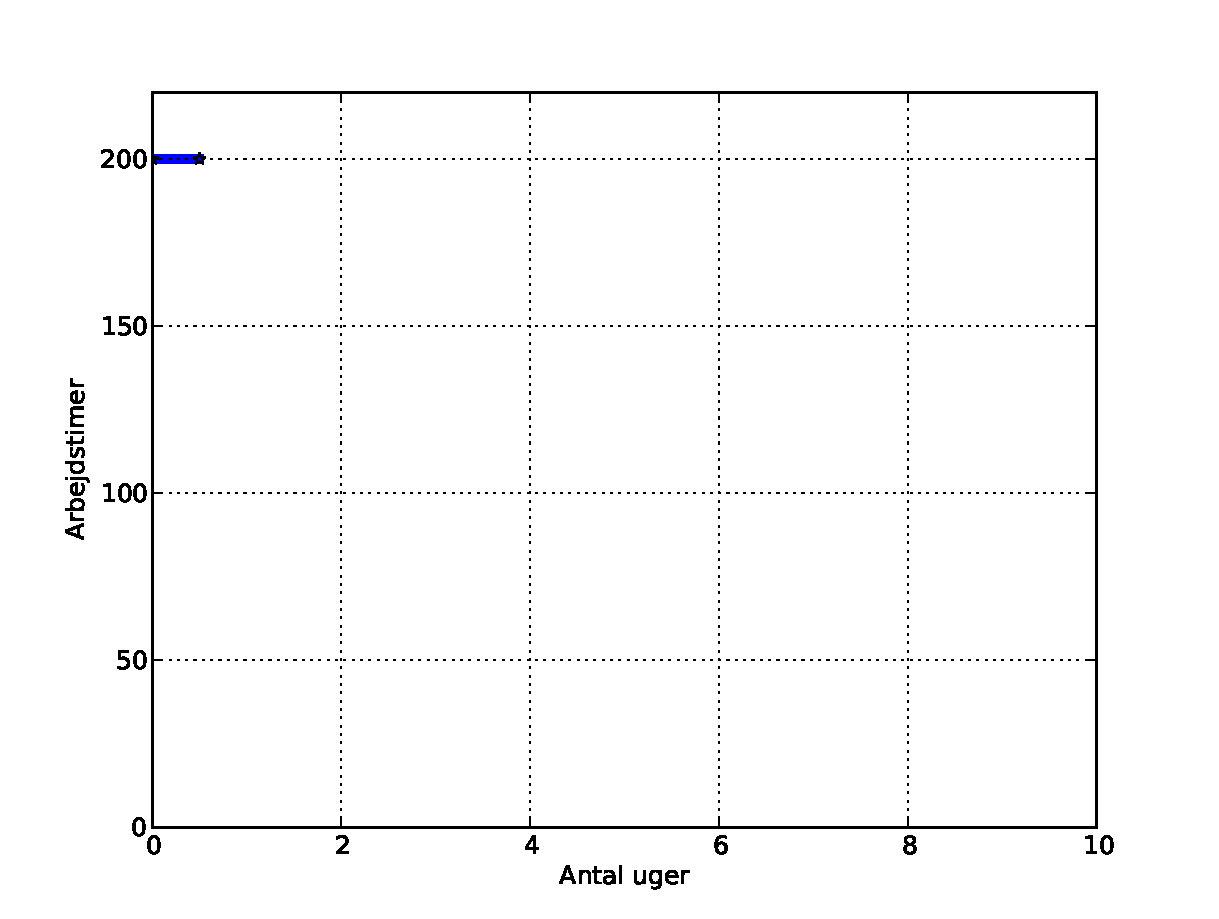
\includegraphics[width=15cm, height=12cm]{burndown.pdf}
\caption{Burndown diagram over projektforløbet}
\label{fig:bd}
\end{figure}

Vi har som udgangspunkt afsat mellem 8 og 10 uger til det agile projektforløb
og bedømt den påkrævede arbejdsindsats til at være 200 timer, hvilket vil sige 100
timer til hver, da vi er to mand i gruppen. Dette overslag er dog yderst
usikkert, men vi har aldrig prøvet at arbejde på denne måde før, så det bliver
spændende at se, om vores estimationer bliver mere præcise undervejs. Vi har
planlagt at udvikle i sprints af 14 dages varighed, men vi kan udvide dette til 3
uger, hvis et af punkterne i produkt backloggen forekommer mere omfangsrigt.\\
Indehaveren af K. Translation har ofte meget travlt og kan som sagt ikke
deltage i hvert nyt sprintmøde. Derfor har vi besluttet at simulere disse
møder ved, at vi selv skriver og opdater produkt backloggen og gør det med
udgangspunkt i kravspecifikationen. Vi bliver herved in effect vores egen 
proxykunde ! Den indledende produkt backlog kan ses i tabel 1.

\begin{center}
	\begin{tabular}{|p{8cm}|l|l|l|}
		\hline
Punkt & Prioritet & Værdi & Indsats \\ \hline
Som bruger af KT's hjemmeside bliver man præsenteret for en kalender, hvori man
kan booke en aftale med KT. & 1 & Høj &     \\ \hline
Som KT's kunde møder man et login interface, når man navigerer til hjemmesiden. & 2 &
Høj & 15  \\ \hline
KT skal have muligheden for løbende at tilføje kunder til databasen. & 3 & Høj
& \\ \hline
Man skal som kunde modtage en bekræftende email efter at have lavet en aftale
i kalenderen. & 4 & Middel &   \\ \hline
Som kunde skal man kunne søge i kalenderen ved hjælp af dato eller klokkeslet.
& 5  & Middel &   \\ \hline
Indehaveren af KT vil gerne kunne synkronisere sin eksterne kalender med
hjemmesidens kalender og på den måde overføre sine private aftale. & 6 & Lav &
\\ \hline
KT ønsker en hjemmeside med kontaktinformation, billeder og et enkelt design.
& 7 & Middel & 12 \\ \hline
\end{tabular}
\caption{\textbf{Tabel 1} Produkt Backlog}
\end{center}
\vspace{0.5cm}

KT's ønsker står i prioriteret rækkefølge, og vi har yderligere tilføjet en
kolonne, hvor KT kan estimere nytteværdien af punktet med Høj, Lav eller
Middel. Sidste kolonne viser vores bedømmelse som udviklere af den påkrævede
arbejdsindsats. Ofte vil punkterne i produkt backloggen være formuleret som
små bruger historier eller endda som deciderede use cases. Dernæst har vi
valgt ud, hvilke punkter vi koncentrerer os om i den første sprint. Dette
fremgår af tabel 2, som er Sprint Backloggen. Punkterne bliver yderligere
delt op i sprint opgaver, og hver udvikler påtager sig et antal opgaver og
kommer igen med en bedømmelse af den påkrævede arbejdsindsats i timer. Sprint
backloggen bliver dermed udgangspuktet for systemudviklingen i den
efterfølgende sprint. 


\begin{center}
	\begin{tabular}{|l|p{4cm}|l|l|}
		\hline
		Backlog punkt & Sprint opgave & Frivillig & Indsats\\ \hline
		\multirow{4}{4cm}{Som KT's kunde møder man et login interface,
		når man navigerer til hjemmesiden.} & Oprette en Django
		applikation & Omar  & 2 \\
		& Skriv login interfacet & Morten & 6 \\
		& Test login interfacet & Omar & 3 \\
		& Integrer interfacet med resten af hjemmesiden & Morten og Omar
		& 4 \\ \hline
		\multirow{3}{4cm}{KT ønsker en hjemmeside med
		kontaktinformation, billeder og et enkelt design.} &
		Skrive basisskabelonen til Django & Morten & 5 \\
		& Udvid basisskabelonen med ``extend''-skabeloner & Morten & 5
		\\ & Test hjemmesiden i flere forskellige browsere & Omar & 2 \\
		\hline

	\end{tabular}
\caption{\textbf{Tabel 2} Sprint Backlog}
\end{center}
		

\section{Anvendelsesområde}
Vi vil i de næste afsnit kigge på to centrale dele af enhver modellering;
nemlig anvendelses- og problemområdet. Vi begynder her med en analyse af
anvendelsesområdet, og for overskuelighedens skyld præsenterer vi det først
ved hjælp af et UML-diagram. Se figur \ref{fig:anvend}.\\

\begin{figure}[!ht]
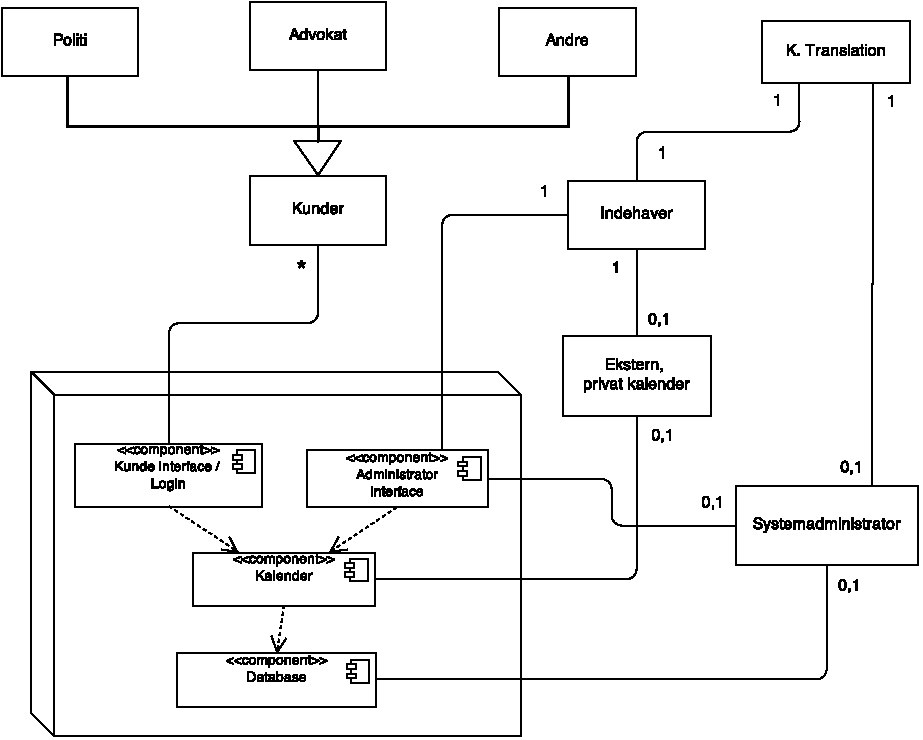
\includegraphics[width=12cm, height=11cm]{anvendelsesomr.pdf}
\caption{UML-diagram over anvendelsesområdet}
\label{fig:anvend}
\end{figure}

Det skal dog præciseres, at det store kvadrat i nederste venstre hjørne i figur
\ref{fig:anvend} ikke hører til anvendelsesområdet. Det er et high-level
billede af problemområdet, som her er medtaget for at binde de to områder sammen,
og som behandles indgående i næste afsnit.\\ 
Umiddelbart er anvendelsesområdet meget begrænset. Vi har fundet følgende
klasser, der skal modelleres i anvendelsesområdet:

\begin{itemize}
\item K. Translation med indehaver (som samtidig er eneste medarbejder)
\item Systemadministrator kos K. Translation
\item K. Translations kunder som politi, advokater, etc.
\item Eksternt, privat kalendersystem 
\end{itemize}

K. Translations indehaver, som samtidig er den eneste medarbejder, skal som
den første modelleres i systemet. Hun skal bruge kalenderen og
bookingssystemet i sit daglige arbejde, og hendes ønske er, at kunne kombinere
hendes private kalender med vores it-løsning, så hun har alle sine aftaler
samlet et sted. Derfor har vi modelleret hende som indehaver af K.
Translation og bruger af kalenderen, men vi har samtidig udvidet modellen med
en ekstern kalenderklasse mellem indehaveren og systemet, hvor hendes private
aftaler ligger, og hvor den eksterne kalender kan synkronisere med vores
bookings- samt kalendersystem og overføre de private aftaler. Det skal dog
siges, at vi på nuværende tidspunkt er meget usikre på denne funktion, og at
vi potentielt må fortælle K. Translation, at dette ligger uden for vores
formåen, så vi er påpasselige med at stille hende for meget i udsigt. Derfor
har den også i UML-diagrammet fået multiplicitet 0, 1, da vi højest regner med
1 ekstern kalender, der skal integreres. Det kunne godt gå hen og blive en stor
og kompliceret opgave, så derfor får den også i første omgang en lavere prioritet 
end andre mere tilgængelige ønsker. Se evt. afsnittet om projektplan.\\
Vi har i UML diagrammet givet indehaveren af KT multiplicitet 1.
Man kunne sagtens forestille sig flere ejere af bureauet, men vi har taget
udgangspunkt i den nuværende situation, og der er ikke umiddelbart udsigt til 
nogen ændringer. Selvom indehaveren ikke besidder it-kundsskaber ud over det
almindelige, har vi i erkendelse af, at hun også er eneste medarbejder, i
UML-diagrammet givet hende adgang til administrationsinterfacet, da hun sikkert
vil komme i en situation, hvor hun selv er nødt til at tilgå systemet med alle
rettigheder for at ændre eller oprette nye kunder. \\
Hvis vi skal foresætte modelleringen af anvendelsesområdet, så er der en
Systemadministratorklasse associeret til K. Translation. Indehaveren af KT
er ganske almindelig it-bruger, og her snakker vi om mail, netbank, facebook,
etc, men er ikke it-kyndig udover dette. Derfor er vi nødt til at modellere en
systemadministrator, der har overblik over systemet, og som kan yde support,
hvis der opstår problemer. Hvis det færdige system ikke kommer til at ligge på
en intern server hos KT, men ender med at blive hosted af en ekstern udbyder 
af serverplads, så vil nødvendigheden af denne klasse mindskes betragteligt,
men der vil altid være et vist behov for central systemadministration hos KT i
tilfælde af ændringer i kontaktinformation eller kalenderbrug med dertil
hørende ændringer i kodebasen og efterfølgende nye upload til serveren. K.
Translation må selv tage stillig til, hvor meget systemadministration der er
nødvendig efter afleveringen og implementeringen af systememet, men vi vil
naturligvis indgå i en dialog med hende omkring dette emne, når det bliver
aktuelt. \\
Den sidste klasse, der skal modelleres i anvendelsesområdet, er KT's kunder og
samarbejdspartnere. Denne klasse er omdrejningspunktet for hele systemet, da
en af hovedpræmisserne for vores it-løsning er, at KT's kunder på en hurtig og
overskuelig måde kan booke en aftale med tolkeservicen. Kundegrundlaget er  
offentlige myndigheder som politi, ministerier og hospitaler samt private
aktører som advokater og andre samarbejdspartnere. Når de møder hjemmesiden, skal
de kunne tilgå kalenderen via et loginsystem med deres EAN-nummer og derfra
føres videre til selve kalenderen, hvor der kan bookes en aftale. Vi må
forvente, at kundesegmentet har meget svingende it-kundsskaber, men at de i
kraft af deres daglige arbejde er vant til at arbejde med diverse login- og 
kalendersystemer, der findes overalt i f.eks. den offentlige sektor. \\

\section{Problemområde}
Efter at vi har modelleret tilgangen til it-systemet gennem
anvendelsesområdet, er turen kommet til systemets hjerte: problemområdet. Det
er her, vi med hjælp af modelleringen senere skal implementere vores
løsninger på KT's krav og ønsker. For at binde modelleringen sammen går alle 
klasserne fra anvendelsesområdet igen i problemområdet. Vi præsenterer igen for
overskuelighedens skyld først et UML-diagram over området. Se figur 
\ref{fig:problem}. Dernæst kommer der en kort opsummerende liste med klasserne 
efterfulgt af et længere forklarende afsnit.  

\begin{figure}[!ht]
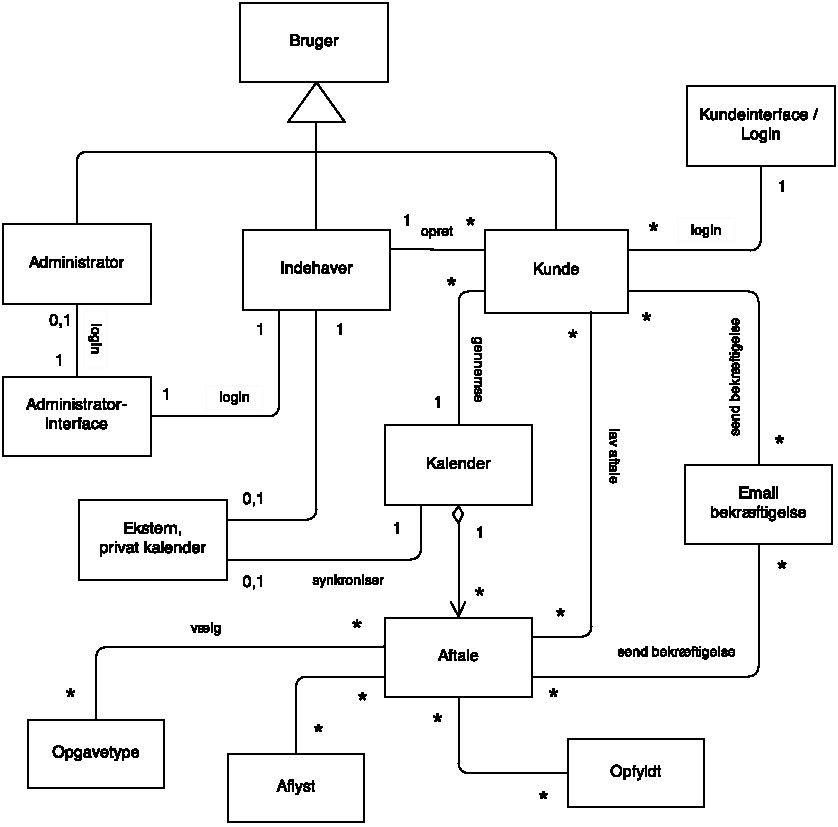
\includegraphics[width=12cm, height=12cm]{problemomr.pdf}
\caption{UML-diagram over problemområdet}
\label{fig:problem}
\end{figure}

Her følger en liste af de klasser vi har identificeret i problemområdet:

\begin{itemize}
\item Bruger: Kunde, administrator, indehaver. Går igen fra
	anvendelsesområdet
\item To interfaces. Et til kunderne og et til administratoren
\item Kalenderen, som kunderne kan bruge, når de skal finde en ledig tid, og
	som KT's indehaver kan bruge i sit daglige, travle arbejde
\item Aftale. Kunderne booker en aftale i kalenderen.
\item En aftale kan både være aflyst og opfyldt, hvis den ikke længere er
	aktuel
\item Når kunden har booket en aftale, sendes der en bekræftende email tilbage
	til kunden med det aftalte tidpunkt
\item KT's indehaver har et ønske om at kunne synkronisere hendes eksterne,
	private kalender med vores it-løsning
\end{itemize}

Vi begynder denne gennemgang af problemområdet med de to interfaces, hvor
brugerne først møder systemet. Systemadministratoren får sit eget selvstændige
interface, idet vedkommende skal kunne tilgå systemet med samtlige
rettigheder. Som vi også nævnte under gennemgangen af anvendelsesområdet, så
skal KT's indehaver alene i kraft af, at hun er eneste medarbejder, også have
adgang til systemet gennem administratorinterfacet. Det betyder også, at vi efter
implementeringen er nødt til at undervise hende grundigt i brugen, og at vi
fabrikerer nogle enkle og præcise manualer, hun efterfølgende kan slå op i.
KT's kunder vil også blive præsenteret for et login interface, når de
navigerer til hjemmesiden. Efter login vil der være adgang til kalender og
bookingsystemet. \\
Omdrejningspunktet i problemområdet må siges at være kalenderen, da hele
systemets berettigelse hviler på denne. Vi skal have fundet en eller anden
kalenderform, der passer til opgaven og KT's arbejdsgange. Indehaveren af K.
Translation har som udgangspunkt fortalt, at der ikke forekommer aftaler længere
end 2-3 uger ude i fremtiden, men det vil også være for meget for en
almindelig computerskærm at skulle vise to eller tre hele kalenderuger med
aftaler, så derfor er vi nødt til at finde et acceptabelt kompromis på,
hvordan kalenderen skal præsenteres. Vi kunne begynde med at vise kunden dags 
dato og inkorporere søgefunktioner på dag, uge og klokkeslet, men det endelige
design er på nuværende tidspunkt ikke fastlagt.\\
Det er også et krav til kalenderen, at kunden let kan skelne mellem ledige
tidspunkter og allerede bookede aftaler ved hjælp af et farvesystem. Her vil
ledige tidspunkter være markeret med grøn skrift og aftaler med rød skrift. \\
Dette fører modelleringen af problemområdet videre til aftale klassen. Der vil 
være en naturlig sammenhæng mellem kalender og aftale, og derfor er de
sammenkoblet ved aggregering. En kunde kan lave en eller flere aftaler på
samme tid, og vedkommende vil efter hver indgået aftale automatisk modtage en 
bekræftende email med dato og tidspunkt. Dette ses til højre i UML-diagrammet,
hvor emailen autogeneres og sendes tilbage til kunden. Vi har suppleret aftale
klassen med to tilhørende klasser: aflyst og opfyldt, som er de to tilstande,
en aftale kan være i. (En igangværende aftale har vi ikke fundet vigtig nok
til at modellere). Der skal i kalenderen være mulighed for at aflyse en
allerede indgået aftale, og proceduren vil være den samme som ved oprettelsen.
Kunden logger på, aflyser aftalen og modtager en autogeneret email som
bekræftigelse. Hvorvidt kunden er interesseret i at beholde gamle og udløbne aftaler 
i kalenderen, står endnu ikke helt klart. De kunne bibeholdes som en form for
kalenderhistorie eller logbog, hvis KT skal gennemgå gamle aftaler i
forbindelse med fakturering eller anden opgørelse, men det ville være mest
hensigtsmæssigt at sætte en grænse, så databasen ikke fyldes op med gamle,
ligegyldige aftaler.\\ 
Det sidste, vi vil berøre i problemområdet, er det usikre punkt om samspillet
mellem en ekstern kalender og vores eget kodede kalendersystem. KT's indehaver
har sin egen private Google kalender, som hun gerne vil synkronisere med vores
it-løsning for at overføre hendes private aftaler, så alt er samlet i en
kalender. Det ville være en smuk løsning at kunne implementere noget sådant,
men vi er nødt til seriøst at overveje kompleksiteten af dene opgave. Måske må
vi stille K. Translation i udsigt, at private aftaler skal indtastes manuelt i
kalenderen, men det må vi tage stilling til, når kernefunktionerne er
implementerede. \\
Hermed slutter vi gennemgangen af anvendelses- og problemområdet. Den
ovenstående modellering vil ligge til grund for det videre design og endelige


\section{Softwarearkitektur}
Det kan være en stor udfordring, at finde den rigtige softwarearkitektur i et
systemudviklingsprojekt. Vi har selv overvejet flere forskellige arkitekturer 
og vil i dette afsnit argumentere for vores valg og fravalg. Først overvejede
vi en multilagdelt arkitektur i form af 3-tier arkiekturen. Her kunne vi i
datalaget gemme de oprettede brugere og bookede aftaler i en database.
Forretningslogikken kunne placeres i mellemlaget og kodes med PHP.
Brugerinterfacet ville ligge i præsentationslaget og tilgås gennem brugerens
browser. Vi fravalgte dog denne løsning af flere grunde. Vi fandt det ikke
streng nødvendigt med tre lag, da det tredie lag ikke ville betyde
nævneværdige forbedringer i forhold til en almindelig client-server model.
Derudover kunne vi også uforvarent komme til at introducere flere
sikkerhedsbrister, hvis vi havde kodet mellemlaget i PHP, da dette kræver, at 
man er ekstrem opmærksom på validering af brugerinput. Én maliciøs SQL-injection
kan slette en hel database og alle aftaler, hvilket vil være katastrofalt for
KT. Da vores kalendersystem ikke kræver andet for at fungere end en bruger med
en browser, der kan logge på KT's server, besluttede vi derfor, at holde 
arkitekturen så overskuelig som mulig ved at bruge client-server modellen. \\
Dernæst valgte vi det Model-View-Controller (MVC) baserede web framework Django til
at understøtte client-server arkitekturen. Se figur \ref{fig:mvc}.\\

\begin{figure}[!ht]
	\centering
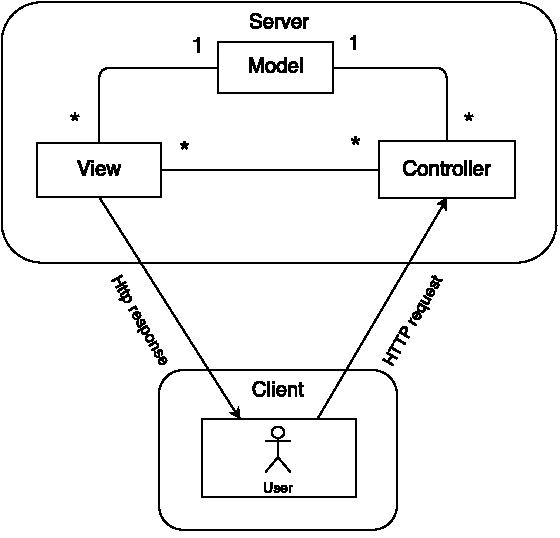
\includegraphics[width=10cm, height=9cm]{mvc.pdf}
\caption{Model-View-Controller arkitektur superimposeret på client-server}
\label{fig:mvc}
\end{figure}

Django kommer med et enkelt og praktisk administratorinterface, der kan blive
særdeles nyttig for os under systemudviklingen og for indehaveren af KT på
længere sigt. Desuden får vi mulighed for at benytte Django's mange indbyggede 
applikationer. Vi kommer til at bruge moduler, der understøtter implementering af
html formularer, og som også er i stand til at validere brugerinput i disse,
og moduler for brugeroprettelse og autentifikation. Det betyder, at der er
færre muligheder for os, til at introducere fejl og sikkerhedsmangler til
systemet. En af Djangos helt store styrker, som udspringer af MVC arkitekturen,
er den løse kobling og strenge adskillelse mellem de forskellige dele af modellen.
Det betyder, at vi let kan ændre, slette eller tilføje i eksisterende dele uden at
bekymre os om afhængigheder mellem delene. \\
Fordi views i Django terminologi består af templates, og controllers består af
viewfunktioner, er det måske mere rigtigt at kalde Django for en Model-View-Templates
(MTV) arkitektur, men vi bibeholder den normale konvention og skriver MVC. Vores
model kommer til at bestå af de aftaler, som KT's kunder booker ind i kalenderen.
D.v.s at domænerne i den bagvedliggende database, som modellen kortlægges til og 
fra, udgøres af datoen og klokkeslettet for aftalen plus anden tilhørende
information. Django's templates står som sagt for præsentationen, og vi
påtænker at bruge en basisskabelon til hjemmesiden, der kan udvides med
tilpassede templates, når logikken kræver det. Selve forretningslogikken, der
er systemet hjerte, bliver implementeret i Django's viewfunktioner.
(Controller i MVC). Det er bindeleddet mellem modellen og præsentationen, og
det er her kernefunktionaliteten kommer til at sidde. Eftersom Django i
virkeligheden er en samling Python biblioteker, vil vi kode systemet i
programmeringssproget Python. Det er også et godt valg, fordi det ene medlem i
vores tomandsgruppe har erfaring med Python, og det andet medlem ikke har.
Python kan læres relativt hurtigt, så det ene medlem får muligheden for at
lære det undervejs i projektet, mens det andet medlem kan lære det fra sig
evt. med pair-programming. \\ 


\section{Use-cases}
\section{Projektplan}

\section{No silver bullit}
\section{ den anden artikel}


\begin{thebibliography}{9}
	\bibitem{oose}
		Bernd Bruegge and Allen H. Dutoit,
		\emph{Object-Oriented Software Engineering Using UML, Patterns
		and Java}.
		Pearson Education Limited, Edinburgh,
		Third Edition,
		2014.
	\bibitem{scrum}
		Jeff Sutherland,
		\emph{Jeff Sutherland's Scrum Handbook}
		Scrum Training Institute, Massachusetts,
		Årstal: ?.
\end{thebibliography}

\end{document}











